\documentclass{article}

\title{Notes: Stretch Mapping}
\author{D. Fang}
\date{\today}

\usepackage{amsmath, amssymb}
\usepackage{derivative}
\usepackage{tikz}
\usepackage{hyperref}
\usepackage{tcolorbox}
\usepackage{empheq}

\newcommand{\me}{m_\mathrm{e}}
\newcommand{\mpr}{m_\mathrm{p}}
\newcommand{\mue}{\mu_\mathrm{e}}
\newcommand{\tpf}{\tilde{p}_F}
\newcommand{\Mtot}{M_{\text{tot}}}
\newcommand{\xmax}{x_{\max}}
\newcommand{\dr}{\odif{r}}
\newcommand{\Rsun}{R_{\odot}}
\newcommand{\Msun}{M_{\odot}}
\newcommand{\Tsun}{T_{\odot}}
\newcommand{\uiv}{u_{\textrm{IV}}}
\newcommand{\ucv}{u_{\textrm{CV}}}
\newcommand{\rhoIV}{\rho_{\textrm{IV}}}
\newcommand{\cs}{c_{\textrm{s}}}
% \newcommand{a}{a_{\textrm{T}}}
% \newcommand{A}{A_{\textrm{T}}}
% \newcommand{B}{B_{\textrm{T}}}
% \newcommand{b}{b_{\textrm{T}}}
% \newcommand{\alpha}{\alpha_{\textrm{T}}}
% \newcommand{\beta}{\beta_{\textrm{T}}}

\DeclareMathOperator{\arcsinh}{arcsinh}
\DeclareMathOperator{\sinc}{sinc}

\begin{document}

\maketitle
\tableofcontents

\section{Coordonnées}

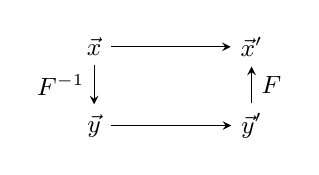
\begin{tikzpicture}[node distance=2cm, >=stealth, every node/.style={font=\small}]

  % positions
  \node (a) at (0,1) {$\vec x$};
  \node (b) at (0,0) {$\vec y$};
  \node (c) at (2,0) {$\vec y'$};
  \node (d) at (2,1) {$\vec x'$};

  % arrows
  \draw[->] (a) -- (b) node[midway, left] {$F^{-1}$};                     % a -> b (down)
  \draw[->] (b) -- (c);                     % b -> c (right)
  \draw[->] (c) -- (d) node[midway, right] {$F$};   % c -> d (up) with label
  \draw[->] (a) -- (d);                     % a -> d

\end{tikzpicture}

La procédure de stretch mapping permet d'obtenir les 3 composantes $\vec y'$ à partir de celles de $\vec y$ de manière indépendante.
\[ y_i' = \xi_i(y_i) \]
On veut ensuite retrouver les composantes dans la base de $\vec x$.
Souvent les changements de bases se factorisent, dans le sens où
\begin{equation}
  x_i = \prod_j F^j_i(y_j)
  \label{eq:initial}
\end{equation}
Par exemple,
\begin{align*}
  x &= r \cos\theta\sin\phi
  \\
  y &= r \sin\theta\sin\phi
  \\
  z &= r\cos\phi
\end{align*}

Donc
\begin{align*}
  x_i' &= \prod_j F^j_i(y_j') \\
  &= \prod_j F^j_i(\xi_j(y_j))
\end{align*}
Le problème ainsi c'est que l'on réalise souvent des étapes en trop. Par exemple si on stretch seulement selon $r$, alors il faut partir de $(x,y,z)$, obtenir  $(r,\theta,\phi)$ puis $(r',\theta,\phi)$ puis revenir à $(x',y',z')$. Le calcul de $\theta$ et $\phi$ est alors inutile puisqu'ils restent inchangés.

Dans ce cas, il suffit de suivre la procédure suivante. On part en fait de \eqref{eq:initial} et on l'injecte dans

\section{Introduction}
On cherche un potentiel pour contrer la pression.

\[ -\nabla P + \nabla \phi_{\text{fictif}} =0 \]
On parle d'équation localement isotherme lorsque la température dépend uniquement de la position. Elle est prescrite. Dans les disques protoplanétaires, on dit en effet qu'elle dépend de la distance à l'étoile.

Eos adiabatique :
\[ \rho = P^\gamma \]

\section{Smoothing length}
On veut imposer
\[ h_a = h_{\text{fact}}\left(\frac{m_a}{\rho_a}\right)^(1/3) \]
Or on donne $ \rho_{\text{profile}}$ tel que
\[ \rho(r) = m_{\text{tot}}   \frac{\rho_{\text{profile}}(r)}{\int_{r_{\min}}^{r_{\max}} \rho_{\text{profile}}(r) \odif{S} \odif{r}}\]

\section{HCP Lattice}
On a un cube dans lequel on place des cellules unités hcp. Chaque cellule est de volume $24\sqrt{2}r$ donc au total on a $\frac{(2\xmax)^3}{24\sqrt{2}r}$ cellules. Chaque cellule a 6 atomes donc il reste
\[
  \frac{(2\xmax)^3}{4\sqrt{2}\dr^3} \text{ atomes}
\]
Enfin on crop une sphère donc il reste
\[
  N = \frac{(2\xmax)^3}{4\sqrt{2}\dr^3} \times \frac{\frac43 \pi \xmax^3}{(2\xmax)^3} \text{ atomes}
\]
Dans Shamrock on entre la masse d'une particule:
\[ m_{\text{part}} = \frac{M_{\text{tot}}}{N} \]
où $M_{\text{tot}}$ est la masse de l'étoile que l'on souhaite.
Mais ce serait plus pratique d'entrer $(\Mtot, N, \xmax)$ et d'en déduire $\dr$. On inverse donc
\[ \dr = 2\xmax\left[\frac{1}{4\sqrt2 N}\times\frac{\frac43 \pi}{2^2} \right]^{\frac13}\]

\subsection{Relation masse rayon}
On veut connaître maintenant le lien entre xmax et la masse totale de l'étoile puisqu'a la fin on ne précise que xmax et dr.
Le rayon d'une naine blanche est celle qui maximise ? l'energie libre ?
\[
R_* = \frac{(9\pi)^{2/3}}{8} \frac{\hbar^2}{\me} \frac{1}{G m_p^{5/3} M_{\text{tot}}^{1/3}}\]

\[
  \frac{R_*}{\Rsun} = 0.010\left( \frac{\Msun}{\Mtot}\right)^{\frac13}
\]
Plus l'étoile est massive, plutôt elle doit être petite.

\subsection{Polytrope}
Pour une étoile polytropique. On suit la même procédure. On impose la masse, le rayon est alors contraint.

On donne $\Mtot, \tilde\rho$.
Alors avant de démarrer la procédure de stretch mapping il faut connaître le rayon.
\[
  \Mtot = \int_{0}^{R} \rho_c \tilde\rho(r)4\pi\odif{r}^2
\]
mais donc il faut connaître $\rho_c$. Il nous faut une 2ème équation. Le profil de densité, peu importe son facteur de normalisation doit s'annuler en $R$.
\[
  \tilde \rho(R) = 0
\]
ce qui impose $R$. On pourrait croire que cette équation suffit pour avoir $R$. Mais en fait $\rho_c$ apparaît dedans en raison de l'adimensionnement des équations de Lane-Emden
\[  \tilde \rho(r) = \sinc(\xi(r,\rho_c))\]
avec
\[ \xi(r,\rho_c) =  r\sqrt{\frac{4\pi G\rho_c^2}{(n+1)P_c}} =  r\sqrt{\frac{4\pi G\rho_c^{1-\frac1n}}{(n+1)K}}\]
Finalement, le couple d'équations est
\begin{align}
  0 &=  \tilde \rho(R, \rho_c) \\
  \Mtot &= \int_{0}^{R} \rho_c \tilde\rho(r)4\pi\odif{r}^2
\end{align}
En particulier pour $n=2$,
\[
0 = \sinc\left(R\sqrt{\frac{2\pi G}{K}}\right) \quad \textit{(on a de la chance que $\rho_c$ disparaisse...)} \]
\begin{align*}
  R &= \sqrt{\frac{\pi K}{2 G}} \\
  \Mtot &= \rho_c \int_{0}^{\sqrt{\frac{\pi K}{2 G}}}  \tilde\rho(r)4\pi\odif{r}^2
\end{align*}
tl:dr. Pour $n=1$, c'est la valeur de $K$ uniquement qui impose le rayon. La seule chose qu'on impose c'est $\Mtot$ (donc $N_{\text{part}}, m_{\text{part}}$). $\rho_c$ n'a aucune importance ici.

Résumé :
$R, \Mtot$ sont directement liés.
\begin{itemize}
  \item Fermi : On impose $y_0$ qui impose $\Mtot, R$  directement.
  \item Polytrope : On impose $K,n=1$ ce qui contraint $R$. Puis $\Mtot$ arrive en dernier. Sinon on peut faire l'inverse : imposer $R$ ce qui contraint $K$.
  \item Dans le cas général (par ex Tillotson), on impose le rayon ce qui impose la masse totale ou inversément.
\end{itemize}
% \[ R_*^{\text{polytrop}} = \sqrt{\frac{\pi K}{2G}} \]
% En fait en général
% \[ R_*^{\text{polytrop}} = \sqrt{\frac{(n+1)P_c}{4\pi G \rho_c^2}}\xi_1 \]
% $\xi_1$ étant le point où la densité s'annule.
% avec
% \[ \xi = r\sqrt{\frac{4\pi G\rho_c^2}{(n+1)P_c}} \]

\section{Équations d'état}
\subsection{Fermi}

Par définition de la vitesse du son
\[ c_s^2 \equiv \pdv{P}{\rho} \]
Dans le cas de Fermi,
\[ c_s^2 = \pdv{P}{\tpf}\pdv{\tpf}{\rho}\]
avec
\begin{align*}
  \tpf &= \frac{1}{\mue^{\frac13}}\alpha \rho^{1/3} \\
  P &= \beta \left(\left[\tpf\sqrt{\tpf^2+1}(2\tpf^2-3)+3\arcsinh(\tpf)\right]\right)
\end{align*}
et
\begin{align*}
  \alpha &= \frac{1}{\me c}h\left(\frac{3}{8\pi m_{\mathrm{p}}}\right)^{\frac13} \\
  \beta &= \frac{\pi m_\mathrm{e}^4c^5}{3h^3}
\end{align*}
Donc chaque dérivée donne
\begin{align*}
  \pdv{\tpf}{\rho} &= \frac{1}{3\mue^{\frac13} }\alpha\rho^{\frac13-1} \\
  \pdv{P}{\tpf} &= \beta\Bigg\{\sqrt{\tpf^2+1}(2\tpf^2-3) + \tpf\left[\frac{\tpf}{\sqrt{\tpf^2+1}}(2\tpf^2-3) + 4\tpf\sqrt{\tpf^2+1}\right]  \\
  & \quad + \frac{3}{\sqrt{1+\tpf^2}} \Bigg\} \\
  &= \beta\Bigg\{\frac{1}{\sqrt{1+\tpf^2}}\Bigg[\underbrace{(2\tpf^2-3)(1+\tpf^2)}_{-\tpf^2 + 2\tpf^4 - 3}+ \tpf^2\underbrace{\left[2\tpf^2-3 + 4(\tpf^2+1)\right]}_{6\tpf^2+1}\Bigg]
  + \frac{3}{\sqrt{1+\tpf^2}} \Bigg\} \\
  &= \beta\Bigg\{\frac{8\tpf^4 -3}{\sqrt{1+\tpf^2}}
  + \frac{3}{\sqrt{1+\tpf^2}} \Bigg\} \\
  &= \beta\frac{8\tpf^4}{\sqrt{1+\tpf^2}}
\end{align*}
Finalement
\[ c_s^2 = \frac{8\alpha\beta}{3\mue^{\frac13}\rho^{\frac23}}\frac{\tpf^4}{\sqrt{1+\tpf^2}}\]

\begin{tcolorbox}
  \begin{align*}
    P &= \beta \left(\left[\tpf\sqrt{\tpf^2+1}(2\tpf^2-3)+3\arcsinh(\tpf)\right]\right)\\
    c_s^2 &= \frac{8\alpha\beta}{3\mue^{\frac13}\rho^{\frac23}}\frac{\tpf^4}{\sqrt{1+\tpf^2}}
  \end{align*}
  with
  \begin{align*}
    \tpf &= \frac{1}{\mue^{\frac13}}\alpha \rho^{1/3} \\
    \alpha &= \frac{1}{\me c}h\left(\frac{3}{8\pi m_{\mathrm{p}}}\right)^{\frac13} \\
    \beta &= \frac{\pi m_\mathrm{e}^4c^5}{3h^3}
  \end{align*}
\end{tcolorbox}

\section{Equation de Chandrasekhar}

\[
  \frac{1}{\eta^2} \odv{}{\eta} \left( \eta^2 \odv{\Phi}{\eta} \right) = - \left( \Phi^2 - \frac{1}{y_0^2} \right)^{3/2}
\]

Conditions aux limites :
\begin{align*}
  \Phi(0) &= 1 \\
  \Phi'(0) &= 0 \\
\end{align*}

On résout numériquement cette équation puis on repasse dans les bonnes dimensions.

\begin{align*}
  \eta &= \frac{r}{a} \\
  \Phi &= \frac{1}{y_0}\sqrt{1+\frac{\rho}{C}^{\frac23}}
\end{align*}
On inverse
\begin{align*}
  r &= a\eta \\
  \rho &= C\left[(y_0\Phi)^2- 1\right]^{\frac32}
\end{align*}
Les constantes valent
\begin{align*}
  C &= \frac{8\pi\me^3c^3\mpr}{3h^3} \mue = C_1\mue \\
  a &= \frac{1}{C y_0}\sqrt{\frac{2\beta}{\pi G}} = r_a\frac{1}{\mue y_0}
\end{align*}
avec
\[
  r_a = \frac{1}{C_1}\sqrt{\frac{2\beta}{\pi G}}
\]

\section{Pas de temps pour une naine blanche}
On regarde le rapport $\frac{\tau}{\odif{t}_{\min}}$ où $\tau$ est le temps caractéristique de l'évolution de l'étoile et $\odif{t}_{\min}$ le pas de temps imposée par la CFL.
Normalement le $\odif{t}_{\min}$ est au centre
\[
  \odif{t}_{\min} = \frac{h_{\min}}{c_{s,\max}}
\]
puisque $c_s$ est maximal au centre et $h$ minimal.
Le $\tau$ correspond à la traversée d'une onde sonore à travers $R$.
\[
  \tau = \frac{R}{\overline c_s}
\]
Au final,
\[ \frac{\tau}{\odif{t}_{\min}} = \frac{R}{h_{\min}} \frac{c_{s,\max}}{\overline c_s} \approx   \frac{R}{h_{\min}}  \]
car $c_s$ varie à peine d'un facteur $10$ entre $r=[0,R]$.
Ce qui doit correspondre à
\[ \frac{\tau}{\odif{t}_{\min}} \approx N^{\frac13} \]
En effet
\[ h \approx n^{-\frac13} \approx \left(\frac{R^3}{N}\right)^\frac13 \]
Application numérique. Unités du code $(\Msun, \Rsun, \Tsun = \sqrt{\frac{\Rsun^3}{\Msun G}})$ (donc $G=1$). On prend une WD d'à peu près $M=\Msun, R=10^{-2}\Rsun$
Ça donne des $c_s \approx 10$.
En effet, grossièrement à l'équilibre
\[ \frac{P}{R} = \rho \frac{\Msun G}{R^2} \]
D'où
\[c_s \approx \sqrt{\frac{P}{\rho}} \approx \sqrt{\frac{\Msun G}{R}} = \sqrt{\frac{\Rsun}{R}} \frac{\Rsun}{\Tsun} = \sqrt{\frac{\Rsun}{R}} \approx 10 \]
Au final, on s'attend à un $\odif{t}_{\min}$ de
\begin{empheq}[box=\fbox]{align*}
  \odif{t}_{\min} &= \frac{h_{\min}}{c_{s,\max}} \approx \frac{h_{\min}}{10} \\
  \odif{t}_{\min} &= \frac{\tau}{N^{\frac13}} = \frac{R}{\overline c_s N^{\frac13}} \approx \frac{10^{-2}}{10 N^\frac13} \stackrel{N=10^5}{=} [10^{-4},10^{-5}]
\end{empheq}

\section{Tillotson equation}

In the Tillotson EOS thermodynamic phase space is divided into a compressed region $(\rho > \rho_0$)
and an expanded region $(\rho < \rho_0)$, where $\rho, \rho_0$ are the density and zero-pressure density, respectively. The expanded
region is further divided into \textbf{three} subregions, based on the material's internal energy $e$: (1) expanded cold state
$(u < \uiv)$, (2) expanded hot state $(u > \ucv)$, which converges to ideal gas at low densities, and (3) an intermediate
state $(\uiv < e < \ucv)$, known as the mixed phase state. Here, $\uiv$, and $\ucv$ are the energies at incipient vaporization and
complete vaporization, respectively. In Tillotson (1962) the mixed phase state was governed by the same equation as the
expanded cold state. To avoid pressure discontinuities, in modern approaches the mixed phase state is often assigned
an alternative equation, which is simply a linear interpolation of the equations of the expanded subregions (Holian and
Holian, 1989). The interpolation is purely mathematical, and does not represent a physical phase transition. Tillotson
is convenient to implement in hydrocodes, is computationally fast, but suffers from the lack of phase transitions, and
the exclusion of entropy and temperature

We write
\begin{align*}
  \eta &= \frac{\rho}{\rho_0} & \text{(compression)}\\
  \chi &= \eta -1 &\text{(strain)}
\end{align*}
\begin{enumerate}
  \item Compressed region $\rho\geq\rho_0$
    \[p = \left[a + \frac{b}{1+\frac{u}{E_0\eta^2}}\right]\rho u + A \chi + B \chi^2\]
  \item Expanded $(\rhoIV <\rho < \rho_0)$ cold state $(u<\uiv)$
    Same thing
  \item Expanded but completely vaporized $(\rho < \rho_0)$ hot state $(u>\ucv)$
    \[p = a\rho u + \left[\frac{b}{1+\frac{u}{E_0\eta^2}}\rho u + A \chi e^{-\beta\left(\frac{\rho_0}{\rho} -1\right)}  \right] e^{-\alpha \left(\frac{\rho_0}{\rho} -1\right)^2} \]
  \item Between $(\uiv<u<\ucv)$, $(\rhoIV <\rho < \rho_0)$: linear interpolation
    \[
      p = \frac{(u-\uiv)p_3 +  (\ucv-u)p_2}{\ucv - \uiv}
    \]
  \item Low energy expansion $(\rho < \rhoIV, u<\uiv)$
    \[
      p =  \left[a + \frac{b}{1+\frac{u}{E_0\eta^2}}\right]\rho u + A \chi
    \]

\end{enumerate}

\subsection{Soundspeed}
La vitesse du son est définie par
\[
  \cs^2 = \left(\pdv{P}{\rho}\right)_s
\]
Dans le domaine $(P, \rho, u)$
\[
  \odif{P} = \left(\pdv{P}{\rho}\right)_u \odif{\rho} + \left(\pdv{P}{u}\right)_\rho \odif{u}
\]
Donc
\[
  \cs^2 = \left(\pdv{P}{\rho}\right)_u + \left(\pdv{P}{u}\right)_\rho \left(\pdv{u}{\rho}\right)_s
\]
Il faut donc appliquer le premier principe à un processus isentropique dans le domaine $(u, \rho, s)$
\[
  \odif{u} = -P\odif V = -P\odif{\frac{1}{\rho}} = \frac{P}{\rho^2}\odif{\rho}
\]

Finalement
\[\boxed{
    \cs^2 = \left(\pdv{P}{\rho}\right)_u + \frac{P}{\rho^2}\left(\pdv{P}{u}\right)_\rho
}\]
C'est parti
Déjà

\begin{align*}
  \pdv{p}{\rho} &= \pdv{\eta}{\rho}\pdv{p}{\eta} \\
  \pdv{\eta}{\rho} &= \frac{1}{\rho_0} \\
  \pdv{\chi}{\eta} &= 1 \\
  \pdv{\chi^2}{\eta} &= \pdv{(\eta-1)^2}{\eta} = 2(\eta-1) = 2\chi
\end{align*}

\begin{enumerate}
  \item Compressed region $\rho\geq\rho_0$
    \[p = \left[a + \frac{b}{1+\frac{u}{E_0\eta^2}}\right]\rho_0\eta u + A \chi + B \chi^2\]
    Alors
    \begin{align*}
      \pdv{p}{\eta} &=\left[a + \frac{b}{1+\frac{u}{E_0\eta^2}}\right]\rho_0 u  + \frac{u}{E_0}\frac{2}{\eta^3} \left[\frac{b}{\left(1+\frac{u}{E_0\eta^2}\right)^2}\right]\rho_0 \eta u \\ &+A + 2B\chi \\
      \pdv{p}{\rho} &= \left[a + \frac{b}{1+\frac{u}{E_0\eta^2}}\right] u  + \frac{u^2}{E_0}\frac{2}{\eta^2} \left[\frac{b}{\left(1+\frac{u}{E_0\eta^2}\right)^2}\right] + \frac{1}{\rho_0} (A + 2B\chi)
    \end{align*}
    D'autre part
    \begin{align*}
      \pdv{p}{u} &= \left[a + \frac{b}{1+\frac{u}{E_0\eta^2}}\right]\rho -\frac{1}{E_0\eta^2} \left[\frac{b}{\left(1+\frac{u}{E_0\eta^2}\right)^2}\right]\rho u \\
      \frac{p}{\rho^2}\pdv{p}{u} &= \frac{p}{\rho} \left\{ \left[a + \frac{b}{1+\frac{u}{E_0\eta^2}}\right]-\frac{u}{E_0\eta^2} \left[\frac{b}{\left(1+\frac{u}{E_0\eta^2}\right)^2}\right]\right\} \\
      \frac{p}{\rho^2}\pdv{p}{u} &= \frac{p}{\rho} \left\{ \left[a + \frac{b}{\left(1+\frac{u}{E_0\eta^2}\right)^2}\right]\right\}
    \end{align*}
    Finalement,

  \item Expanded $(\rhoIV <\rho < \rho_0)$ cold state $(u<\uiv)$
    Same thing ??
  \item Expanded but completely vaporized $(\rho < \rho_0)$ hot state $(u>\ucv)$
    \[p = a\rho u + \left[\frac{b}{1+\frac{u}{E_0\eta^2}}\rho u + A \chi e^{-\beta\left(\frac{\rho_0}{\rho} -1\right)}  \right] e^{-\alpha \left(\frac{\rho_0}{\rho} -1\right)^2} \]

    On a les dérivées partielles :
    \begin{align*}
      \pdv{p}{u} &= a\rho +  b\rho \left[\frac{\left(1+\frac{u}{E_0\eta^2}\right)-\frac{u}{E_0\eta^2}}{\left(1+\frac{u}{E_0\eta^2}\right)^2}\right] \mathcal{E} \\
      \frac{p}{\rho^2}\pdv{p}{u} &= \frac{p}{\rho} \left\{a + b\frac{1}{\left(1+\frac{u}{E_0\eta^2}\right)^2}\mathcal{E}\right\} \\
      \mathcal{E} &= e^{-\alpha\left(\frac{\rho_0}{\rho}-1\right)^2} = e^{-\alpha X} \\
      X&= \frac{\rho_0}{\rho} -1 = \frac{1}{\eta} -1
    \end{align*}

    \begin{align*}
      \pdv{p}{\eta} &= a\rho_0 u + b\left( \left[\frac{1}{1+\frac{u}{E_0\eta^2}}\right]\rho_0 u + \frac{\frac{2u}{E_0\eta^3}}{\left(1+\frac{u}{E_0\eta^2}\right)^2}\rho u \right)\mathcal{E} \\
      &+ \left( A \left[1 + \chi\frac{\beta}{\eta^2}\right] e^{-\beta X} \right) \mathcal{E} \\
      &+ \left[\frac{b\rho u}{1+\frac{u}{E_0\eta^2}} + A \chi e^{-\beta X} \right] \left(\frac{2\alpha X}{\eta^2}\right)\mathcal{E}
    \end{align*}

    Soit
    \begin{align*}
      \pdv{p}{\rho} &= a u + \mathcal{E}\left( b\left[\frac{1+ \frac{2\alpha X}{\eta}}{1+\frac{u}{E_0\eta^2}} + \frac{2 u }{E_0 \eta^2 \left(1+\frac{u}{E_0\eta^2}\right)^2} \right] u  + \frac{A}{\rho_0} \left(1 + (2\alpha X + \beta)\frac{ \chi}{\eta^2} \right)e^{-\beta X} \right) \\
    \end{align*}

  \item Between $(\uiv<u<\ucv)$, $(\rhoIV <\rho < \rho_0)$: linear interpolation
    \[
      p = \frac{(u-\uiv)p_3 +  (\ucv-u)p_2}{\ucv - \uiv}
    \]
    \begin{align*}
      \pdv{p}{\eta} &= \frac{(u-\uiv)\pdv{p_3}{\eta} +  (\ucv-u)\pdv{p_2}{\eta}}{\ucv - \uiv} \\
      \pdv{p}{u}&= \frac{p_3 - p_2 + (u-\uiv)\pdv{p_3}{u} +  (\ucv-u)\pdv{p_2}{u} }{\ucv - \uiv}
    \end{align*}
    % \item Low energy expansion $(\rho < \rhoIV, u<\uiv)$
    %   \[
    %     p =  \left[a + \frac{b}{1+\frac{u}{E_0\eta^2}}\right]\rho u + A \chi
    %   \]

    % \begin{align*}
    %   \cs^2 &= \left[a + \frac{b}{1+\frac{u}{E_0\eta^2}}\right]u  + \frac{u}{E_0}\frac{2}{\eta^3} \left[\frac{b}{\left(1+\frac{u}{E_0\eta^2}\right)^2}\right] \eta u \\
    %   &+ \frac{1}{\rho_0}(A + 2B\chi) + \frac{P}{\rho^2}\left(\left[a + \frac{b}{1+\frac{u}{E_0\eta^2}}\right]\rho -\frac{1}{E_0\eta^2} \left[\frac{b}{\left(1+\frac{u}{E_0\eta^2}\right)^2}\right]\rho u\right)
    % \end{align*}

    % \[\boxed{
    %   \cs^2 = \left[a + \frac{b}{1+\frac{u}{E_0\eta^2}}\right]\left(u + \frac{P}{\rho}\right) + \frac{u}{E_0\eta^2} \left[\frac{b}{\left(1+\frac{u}{E_0\eta^2}\right)^2}\right] \left(2u - \frac{P}{\rho}\right) + \frac{1}{\rho_0}(A + 2B\chi)}
    % \]
    % En combinant tout

    % \begin{align*}
    %   \cs^2 &= a u + b\left( \left[\frac{1}{1+\frac{u}{E_0\eta^2}}\right] u + \frac{\frac{2u}{E_0\eta^3}}{\left(1+\frac{u}{E_0\eta^2}\right)^2}\eta u \right)\mathcal{E} \\
    %   &+ \frac{1}{\rho_0}\left( A \left[1 + \chi\frac{\beta}{\eta^2}\right] e^{-\beta X} \right) \mathcal{E} \\
    %   & + \left[\frac{b\eta u}{1+\frac{u}{E_0\eta^2}} + \frac{1}{\rho_0}A \chi e^{-\beta X} \right] \left(\frac{2\alpha X}{\eta^2}\right)\mathcal{E} \\
    %   & \frac{p}{\rho} \left\{a + b\frac{1}{\left(1+\frac{u}{E_0\eta^2}\right)^2}\mathcal{E}\right\}
    % \end{align*}

    % Finalement, la vitesse du son :
    % \[
    %   \boxed{
    %     \begin{aligned}
    %       \cs^2 &= a u + \frac{p}{\rho} \left( a + \frac{b}{\left(1+\frac{u}{E_0\eta^2}\right)^2} \mathcal{E} \right) \\
    %       &+ \mathcal{E}\left( b\left[\frac{1+\frac{2\alpha X}{\eta^2}}{1+\frac{u}{E_0\eta^2}} + \frac{2 u}{E_0 \eta^3 \left(1+\frac{u}{E_0\eta^2}\right)^2} \right]\eta u  + \frac{A}{\rho_0} \left(1 + \frac{(\beta+2\alpha X) \chi}{\eta^2} \right)e^{-\beta X} \right) \\
    %     \end{aligned}
    %   }
    % \]

\end{enumerate}

\subsection{Initialiser une sphère de Tillotson}
\subsubsection{Cas général}

\begin{align*}
  \frac{1}{r^2}\odv{}{r}\left(\frac{r^2}{\rho}\odv{p}{r}\right) &= -4\pi G\rho \\
  p &= \left[a + \frac{b}{1+\frac{u}{E_0\eta^2}}\right]\rho u + A \chi + B \chi^2
\end{align*}

La première équation s'écrit
\begin{align*}
  \odv{}{r}\left(\frac{1}{\rho}\odv{p}{r}\right) + \frac2r\frac{1}{\rho}\odv{p}{r} &= -4\pi G\rho \\
  \odv{}{r}\left(\frac{1}{\rho}\odv{p}{r}\right) + \frac2r\frac{1}{\rho}\odv{p}{r} &= -4\pi G\rho \\
  \left[-\frac{\odv{\rho}{r}}{\rho^2}\odv{p}{r} + \frac{1}{\rho}\odv[order=2]{p}{r}\right] + \frac2r\frac{1}{\rho}\odv{p}{r} &= -4\pi G\rho \\
  \odv[order=2]{p}{r}  + \left(\frac2r -\frac{\odv{\rho}{r}}{\rho}\right) \odv{p}{r} &= -4\pi G\rho^2 \\
\end{align*}
Or
\[
  P=P(\rho)
\]
Donc
\begin{align*}
  \odv{p}{r} &= \odv{p}{\rho}\odv{\rho}{r}\\
  \odv[order=2]{P}{r} &= \odv{p}{\rho}\odv[order=2]{\rho}{r} + \odv{}{r}\left(\odv{p}{\rho}\right)\odv{\rho}{r} \\
  & = \odv{p}{\rho}\odv[order=2]{\rho}{r} + \odv[order=2]{P}{\rho}\left(\odv{\rho}{r}\right)^2
\end{align*}

Finalement
\begin{align*}
  \odv{p}{\rho}\odv[order=2]{\rho}{r} + \odv[order=2]{P}{\rho}\left(\odv{\rho}{r}\right)^2 + \left(\frac2r -\frac{\odv{\rho}{r}}{\rho}\right) \left(\odv{p}{\rho}\right)\left(\odv{\rho}{r}\right) &= -4\pi G\rho^2
\end{align*}
De manière plus lisible,
\begin{align*}
  p'\odv[order=2]{\rho}{r} + p''\left(\odv{\rho}{r}\right)^2 + p'\left(\frac2r -\frac{\odv{\rho}{r}}{\rho}\right) \left(\odv{\rho}{r}\right) &= -4\pi G\rho^2
\end{align*}

Sous forme vectorielle
\begin{align*}
  \mu&=\rho\\
  \nu&=\odv{\rho}{r}\\
\end{align*}
\begin{align*}
  \odv{\mu}{r} &= \nu \\
  p'(\mu) \odv{\nu}{r} + p''(\mu)v^2 + p'(\mu)\left(\frac2r -\frac{\nu}{\mu}\right)v &= -4\pi G \mu^2
\end{align*}

Finalement,
\begin{align*}
  \odv{\mu}{r} &= \nu \\
  \odv{\nu}{r} &=  \left(\frac{\nu}{\mu}-\frac2r\right)\nu - \frac{p''(\mu)}{p'(\mu)}\nu^2  - \frac{1}{p'(\mu)}4\pi G \mu^2
\end{align*}

Il reste les conditions aux limites.
Si on connaît déjà le rayon final alors simplement :
\begin{align*}
  \rho(R_{\max}) &= 0
\end{align*}
Sinon on impose une densité arbitraire au centre
\begin{align*}
  \rho(0) &= \rho_a
\end{align*}
et le rayon est alors déterminé par l'annulation de $\rho$.

\subsubsection{Application à Tillotson}
On part d'une sphère condensée
\begin{align*}
  p &= \left[a + \frac{b}{1+\frac{u}{E_0\eta^2}}\right]\rho u + A \chi + B \chi^2
  \pdv{p}{\rho} \\
  \pdv{p}{\rho} &= \left[a + \frac{b}{1+\frac{u}{E_0\eta^2}}\right] u  + \frac{u^2}{E_0}\frac{2}{\eta^2} \left[\frac{b}{\left(1+\frac{u}{E_0\eta^2}\right)^2}\right] + \frac{1}{\rho_0} (A + 2B\chi) \\
  \rho_0 \pdv[order=2]{p}{\rho} &= \left[\frac{2\frac{u}{E_0 \eta^3} bu}{\left(1+\frac{u}{E_0\eta^2}\right)^2}\right]  + b\frac{u^2}{E_0}\frac{2}{\eta^2} \left[\frac{4\frac{u}{E_0 \eta^3}}{\left(1+\frac{u}{E_0\eta^2}\right)^3}\right] - \frac{u^2}{E_0}\frac{4}{\eta^3} \left[\frac{b}{\left(1+\frac{u}{E_0\eta^2}\right)^2}\right]+ \frac{2B}{\rho_0}  \\
  & =  \frac{8b\frac{u^3}{E_0^2 \eta^5}}{\left(1+\frac{u}{E_0\eta^2}\right)^3} -  \frac{2b \frac{u^2}{E_0\eta^3}}{\left(1+\frac{u}{E_0\eta^2}\right)^2}+ \frac{2B}{\rho_0}
\end{align*}

\subsubsection*{Problèmes}

\begin{enumerate}
  \item Tillotson ne permet pas de récupérer la température donc j'impose temperature uniforme ($u=0$ partout)
  \item En dessous d'une certaine densité ($\rho \lesssim  0.95\rho_0$) la pression devient négative. Domaine non pris en compte par Tillotson ? Correspond à une situation non physique donc j'impose $P=0$ et le rayon de la sphère est le rayon où $P$ s'annule.
  \item Problème qui suit : la densité n'est pas encore nulle au moment la pression s'annule. Il vaudrait mieux qu'il y ait une discontinuité de densité donc j'étends un peu au dela du rayon initial et j'y fixe $\rho=10^{-6}$.
\end{enumerate}

\end{document}
